\documentclass[10pt]{article}
\usepackage{icmlko}

\icmlmeta{IP 파운데이션 월드모델}{226}{트리는 이웃에게 못 빌린다}{웹툰에서만 트리가 지는 까닭을 물었더니 웹툰 이야기가 아니었다. 트리는 혼자로는 어디서나 이기고, 풀링에서 능형만 움직인다}

\begin{document}

\twocolumn[
\icmlheader

\begin{abstract}
노트 225가 ``웹툰에서 트리가 선형에 $-$0.056 진다''를 남기고 왜인지를 물었다.
쟀다 --- \textbf{웹툰 탓이 아니다.} 웹툰만 떼어 혼자 학습시키면 \textbf{트리가
$+$0.0472 로 이긴다}($+$0.3239 대 $+$0.2767). 풀링하면 $-$0.0530 으로
뒤집힌다. 네 도메인을 다 재니 \textbf{트리는 혼자로는 어디서나 이긴다}
--- 세계애니 $+$0.0776 · 웹툰 $+$0.0472 · 애니 $+$0.0311 · 모바일
$+$0.0165. \textbf{갈리는 것은 풀링에서 누가 얼마나 얻느냐다.} 능형의
풀링 이득이 혼자 $\rho$ 와 \textbf{완전 역순}이다(스피어만 $-$1.00):
웹툰(혼자 0.2767) $+$0.1124 · 애니(0.4242) $+$0.0274 · 세계애니(0.4569)
$+$0.0160 · 모바일(0.5160) \textbf{$-$0.0504}. \textbf{트리는 거의
무반응이다} --- $+$0.0122 · $+$0.0160 · $-$0.0046 · $+$0.0006 으로 폭이
0.021 이다. \textbf{풀링은 능형에게 축소이고 트리에게는 거의 아무것도
아니다} --- 능형은 도메인 절편만 따로 두고 계수를 나눠 쓰므로 혼자 못
배우는 도메인이 이웃에게서 빌리는데, 트리는 도메인 지시자로 다시 갈라
버려 빌릴 것이 없다. 그러면 판의 트리$-$선형이 정확히 분해된다:
\textbf{트리$-$선형(풀링) $=$ 트리$-$선형(혼자) $-$ (능형 이득 $-$ 트리
이득)}. 웹툰은 $+$0.0472 $-$ 0.1002 $=$ $-$0.0530 이고 관측과 소수
넷째 자리까지 같다. 네 도메인 모두 맞는다. \textbf{웹툰이 유일하게
뒤집히는 까닭은 혼자 $\rho$ 가 0.2767 로 유일하게 낮아서다} --- 능형이
빌릴 것이 제일 많은 도메인이고, 그 이득이 트리의 혼자 우위를 넘어선다.
\textbf{노트 225가 ``라벨 성질''로 부른 것도, 이 노트가 ``웹툰''으로 부를
뻔한 것도 아니다 --- 혼자 $\rho$ 다.}
\end{abstract}
]

\begin{figure*}[t]
\centering
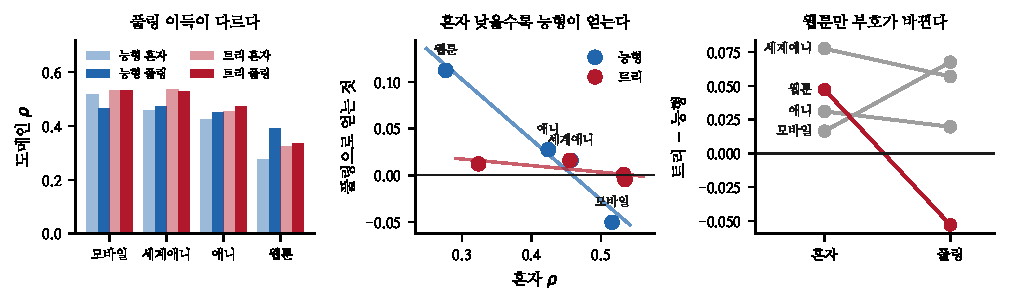
\includegraphics[width=\textwidth]{figs/borrowing.pdf}
\caption{왼쪽 --- 풀링 이득이 모형마다 다르다. 가운데 --- 혼자 낮을수록
능형이 얻는다. 오른쪽 --- 웹툰만 부호가 바뀐다.}
\end{figure*}

\section{웹툰 탓이 아니다}

\begin{table}[t]
\centering\tsize
\caption{도메인 하나만 떼어 학습시키면(노트 222의 채택 상태).}
\begin{tabular}{llrrr}
\toprule
& & 능형 & 트리 & 트리$-$능형 \\
\midrule
\textbf{웹툰} & 혼자 & .2767 & .3239 & \textbf{$+$.0472} \\
& 풀링 & .3891 & .3361 & \textbf{$-$.0530} \\
애니 & 혼자 & .4242 & .4553 & $+$.0311 \\
& 풀링 & .4516 & .4713 & $+$.0197 \\
세계애니 & 혼자 & .4569 & .5345 & $+$.0776 \\
& 풀링 & .4729 & .5299 & $+$.0570 \\
모바일 & 혼자 & .5160 & .5326 & $+$.0165 \\
& 풀링 & .4656 & .5332 & $+$.0676 \\
\bottomrule
\end{tabular}
\end{table}

\claimx{\textbf{트리는 혼자로는 네 도메인 전부에서 이긴다}($+$0.017$\sim$
$+$0.078). 웹툰도 $+$0.0472 다.}{\textbf{그러니 ``웹툰에서 트리가 진다''는
웹툰의 성질이 아니다} --- 풀링했을 때만 그렇다. 노트 225가 라벨 성질을
떼고 남긴 ``웹툰 하나''도 아직 이름이 틀렸다.}

\section{능형만 움직인다}

\begin{table}[t]
\centering\tsize
\caption{풀링으로 얻는 것.}
\begin{tabular}{lrrr}
\toprule
& 혼자 $\rho$(능형) & 능형 이득 & 트리 이득 \\
\midrule
\textbf{웹툰} & \textbf{.2767} & \textbf{$+$.1124} & $+$.0122 \\
애니 & .4242 & $+$.0274 & $+$.0160 \\
세계애니 & .4569 & $+$.0160 & $-$.0046 \\
\textbf{모바일} & \textbf{.5160} & \textbf{$-$.0504} & $+$.0006 \\
\midrule
\multicolumn{2}{l}{혼자 $\rho$ 와의 스피어만} & \textbf{$-$1.00} & --- \\
\bottomrule
\end{tabular}
\end{table}

\claimx{\textbf{능형의 풀링 이득이 혼자 $\rho$ 와 완전 역순이다}
(스피어만 $-$1.00, 넷 다). 혼자 못 배우는 도메인일수록 크게 얻고, 잘
배우는 모바일은 오히려 $-$0.0504 잃는다.}{\textbf{트리는 거의
무반응이다} --- 폭이 0.021 이고 부호도 섞인다. \textbf{풀링은 능형에게
축소이고 트리에게는 거의 아무것도 아니다.}}

\claimx{\textbf{까닭은 두 모형이 ``푸는'' 방식이다.} 능형은 도메인 절편만
따로 두고 \emph{계수를 나눠 쓴다} --- 혼자 못 배우는 도메인이 이웃에게서
빌린다. \textbf{트리는 도메인 지시자로 다시 갈라 버려 빌릴 것이
없다.}}{이전에 잰 압축 법칙(풀링 $=$ 0.127 $+$ 0.688 $\times$ 혼자)이
\emph{능형에만} 적용되는 법칙이었다 --- 그때는 모형을 하나만 놓고 재서
그것이 안 보였다.}

\section{분해가 맞는다}

\claimx{\textbf{트리$-$선형(풀링) $=$ 트리$-$선형(혼자) $-$ (능형 이득
$-$ 트리 이득).}}{웹툰 $+$0.0472 $-$ 0.1002 $=$ $-$0.0530 · 애니
$+$0.0311 $-$ 0.0114 $=$ $+$0.0197 · 세계애니 $+$0.0776 $-$ 0.0206 $=$
$+$0.0570 · 모바일 $+$0.0165 $+$ 0.0510 $=$ $+$0.0675. \textbf{넷 다
관측과 소수 넷째 자리까지 맞는다.}}

\claimx{\textbf{웹툰이 유일하게 뒤집히는 까닭은 혼자 $\rho$ 가 0.2767 로
유일하게 낮아서다} --- 능형이 빌릴 것이 제일 많은 도메인이고, 그 이득
$+$0.1124 가 트리의 혼자 우위 $+$0.0472 를 넘어선다.}{\textbf{이름이
세 번 바뀌었다} --- 노트 224 ``라벨 성질'' $\to$ 노트 225 ``웹툰'' $\to$
이 노트 ``혼자 $\rho$''. \textbf{그리고 이번 것은 넷을 다 설명하고
분해가 닫힌다.}}

\begin{table}[t]
\centering\tsize
\caption{남은 것.}
\begin{tabular}{ll}
\toprule
\textbf{빌리는 트리} & 도메인 간 축소를 트리에 넣을 수 있나 \\
\textbf{손익분기} & 능형 이득이 0 이 되는 혼자 $\rho$ 는 0.44 근처 \\
나머지 여섯 & 작은 도메인에서도 법칙이 서나 \\
\bottomrule
\end{tabular}
\end{table}

첫 줄이 곧바로 값이 크다. \textbf{트리가 혼자로는 어디서나 이기는데
풀링에서 못 얻는다면, 트리에 축소를 붙이면 둘의 좋은 쪽만 가질 수 있다.}
제일 값싼 형태는 \emph{잔차 위의 트리}다 --- 풀링 능형을 먼저 적합해
도메인 간에 빌린 뒤, 그 잔차를 트리로 잡는다. 웹툰에서 능형 풀링이
$+$0.3891 이고 트리 혼자가 $+$0.3239 이므로 \textbf{둘이 서로 다른 것을
잡고 있다면 합이 둘 다보다 클 수 있다.} 그리고 이것은 새 축도 새 수집도
필요 없는 \emph{정식화} 하나다 --- 이 사이클에서 판을 움직인 것이 전부
자료 고침이었으니, 오랜만에 모형 쪽에서 잴 것이 생겼다.

\end{document}
